\documentclass[11pt]{article}

\usepackage[a4paper,margin=1in]{geometry}
\usepackage{indentfirst}
\setlength{\parskip}{0.35\baselineskip plus 1pt minus 2pt}
\raggedbottom
\usepackage{booktabs}
\usepackage{hyperref}
\usepackage{enumitem}
\setlist{
  leftmargin=*,
  topsep=0.35\baselineskip,
  itemsep=0.15ex,
  parsep=0pt,
  partopsep=0pt
}
\usepackage{amsmath}
\usepackage{graphicx}
\usepackage{needspace}
\usepackage{caption}
\captionsetup{skip=4pt, font=small}
\graphicspath{{figures/}}
\newcommand{\reportplot}[1]{%
  \includegraphics[width=\linewidth,height=0.38\textheight,keepaspectratio]{#1}%
}
\usepackage{xcolor}
\usepackage[T1]{fontenc}

\hypersetup{
  colorlinks=true,
  linkcolor=blue,
  citecolor=blue,
  urlcolor=blue
}

\newcommand{\projecttitle}{Cross-Lingual Robustness of Tacit Coordination in LLMs}
\newcommand{\githuburl}{\url{https://github.com/CecilyQE/COMP3520_Project}}
\title{\projecttitle:\\A Human-Referenced Diagnostic Study}
\author{%
  \begin{tabular}{c@{\hspace{4em}}c}
    Huang, Tianxin & Zhang, Jiachang \\
    Student ID: 3036675033 & Student ID: 3036385212 \\[1.5em]
    Lu, Junyu & Li, Juyao \\
    Student ID: 3036675198 & Student ID: 3036678891
  \end{tabular}
}
\date{}

\begin{document}
\maketitle

\begin{abstract}
This project studies whether large language models (LLMs) preserve tacit coordination behavior across instruction languages. We build a human-referenced diagnostic pipeline using pure coordination game items from Perez-Zapata et al. and compare model answer distributions under matched English and Chinese prompts while fixing the required answer language to English. The evaluation separates two questions that are easy to conflate: whether model answers align with human focal-point distributions, and whether the same model remains internally stable across instruction languages. Across 17 finalized Round~1 model runs, cross-lingual stability varies substantially; \texttt{mimo-v2-pro} is the most stable (mean cross-lingual JSD 0.0200, top-1 match 1.0000) and \texttt{gemini-2.5-flash} is closest to the human reference, but no model leads on both axes. A per-model Round~2 retry on flagged mismatch items (16 models, same-model reruns) shows heterogeneous recovery: top-1 agreement improves on 14/31 candidate item--model pairs, but several families (GLM, DeepSeek, \texttt{gpt-5.4}) show little or no gain.
\end{abstract}

\section{Introduction}

Tacit coordination tasks ask participants to choose an answer that they expect another participant will also choose, without explicit communication. These tasks are useful for studying focal points---common, socially salient, or conventionally expected answers \cite{schelling1960,mehta1994,sugden1995}. Recent work suggests that LLMs can participate in such coordination games, but it remains unclear whether their focal-point behavior is robust when the instruction language changes. The question matters beyond single-model benchmarks: in multi-agent workflows, different models---or the same model under different interface languages---are often expected to converge on defaults without explicit negotiation. If focal-point distributions drift across prompt languages, specialized agents in one pipeline may surface incompatible ``obvious'' choices (e.g., different canonical entities, dates, or landmarks), increasing coordination overhead and user correction cost.

We build a reproducible, human-referenced diagnostic pipeline for cross-lingual robustness in tacit coordination. The study has two empirical targets---LLM--human alignment (RQ1) and cross-lingual stability under matched English and Chinese prompts (RQ2)---and an engineering deliverable: a reusable pipeline covering data preparation, prompt generation, sampling, answer normalization, metric computation, and plotting. Round~1 evaluates each model in isolation on the same items; inter-model coordination is left to future work (Section~\ref{sec:futurework}). We do not claim to identify culture as a causal mechanism. Instead, we test whether changing the instruction language, while keeping the answer language fixed, shifts the model's focal-point distribution---a design that avoids confounding instruction-language effects with output-language effects.

Against this backdrop, we ask:
\begin{description}[leftmargin=0.2in,style=nextline]
  \item[RQ1 (Human alignment).]
  How closely do LLM responses match human response distributions on pure coordination items? We report Human-vs-EN and Human-vs-ZH comparisons separately.

  \item[RQ2 (Cross-lingual stability).]
  For the same coordination task and items, how stable are model focal-point distributions across English and Chinese prompts when the required answer language is held fixed to English?

  \item[RQ3 (Exploratory re-coordination).]
  For items that show a first-round cross-lingual top-1 mismatch, can a lightweight second-round retry reduce the mismatch without changing the coordination objective or revealing human distribution information?
\end{description}

The remainder of this report is organized as follows. Section~\ref{sec:related} situates the work relative to prior studies. Section~\ref{sec:methods} covers technical implementation and challenges encountered. Section~\ref{sec:results} presents findings and analysis. Section~\ref{sec:conclusion} summarizes the project, reflection, limitations, and future work. Source code and reproduction instructions: \githuburl

\section{Related Work}
\label{sec:related}

\subsection{Human tacit coordination and focal points}

Schelling introduced the idea that people can coordinate without communication by converging on salient ``focal'' answers \cite{schelling1960}. Mehta, Starmer, and Sugden provide experimental evidence on how salience shapes outcomes in pure coordination games \cite{mehta1994}, and Sugden develops a formal account of why certain answers become focal \cite{sugden1995}. This literature motivates our use of distributional metrics over canonical answers rather than exact string matching alone.

\subsection{Human coordination benchmarks}

Perez-Zapata et al.\ run international pure coordination studies and release item-level human response distributions across panels and countries \cite{perez2026}. We build on their public OSF materials, using the \texttt{study2\_british\_within} panel as a fixed human reference while varying only the instruction language shown to each LLM.

\subsection{LLM tacit and multi-agent coordination}

Aharon et al.\ show that LLMs can participate in tacit coordination games analogous to the human setting \cite{aharon2026}. Agashe et al.\ evaluate broader multi-agent coordination abilities---including pure coordination games and coordination-oriented question answering---and find that performance depends strongly on whether tasks require theory-of-mind-style reasoning about partners \cite{agashe2025coord}. Our study is narrower but complementary: we hold items and sampling fixed and ask whether a \emph{single} model's focal-point distribution is stable across English and Chinese instructions while the required answer language stays English.

\subsection{Multilingual prompting and language confusion}

Multilingual deployment introduces a separate failure mode: models may not follow the intended response language or may shift behavior when prompts mix languages \cite{marchisio2024language}. Marchisio et al.\ show that language confusion is model-dependent and sensitive to prompt complexity. We do not measure response-language violations directly (answers are constrained to English), but their findings motivate treating instruction-language change as a non-neutral intervention rather than a simple translation of labels.

\subsection{Positioning}

Prior human work emphasizes \emph{cross-panel} focal-point variation; prior LLM work emphasizes \emph{whether} models can coordinate. We isolate a third question on the same human-referenced items: \emph{cross-lingual instruction robustness} of a single model's focal-point distribution, reported jointly with human alignment. To our knowledge, few open-ended coordination benchmarks publish both human-referenced alignment and matched EN/ZH stability under a fixed answer language on identical items.

\section{Methods and Technical Implementation}
\label{sec:methods}

We next describe the benchmark panel, evaluation pipeline, normalization protocol, and metrics used in Round~1 and exploratory Round~2 runs.

\subsection{Dataset and Experimental Design}

The human reference data comes from the public pure coordination game dataset of Perez-Zapata et al.\ \cite{perez2026}. The finalized experiments use the \texttt{study2\_british\_within} panel, which contains 15 coordination items and human response distributions. Human answers are aggregated into item-level empirical distributions over canonical answers.

Each item has an English instruction and a curated Chinese instruction. The answer language is fixed to English for both prompt languages. This makes the English-prompt and Chinese-prompt outputs directly comparable in the same answer space.

\subsection{Evaluation Pipeline}

Each model receives matched English and Chinese coordination prompts while the required answer language remains English. Raw responses are normalized to canonical answers and aggregated into item-level distributions; we then compute human-alignment metrics under each prompt language and cross-lingual stability by comparing English- and Chinese-prompt outputs on the same items. Round~2 applies a lightweight retry only when Round~1 shows a cross-lingual top-1 mismatch. Figure~\ref{fig:pipeline} summarizes the workflow: bilingual sampling with a fixed English answer language, canonical-answer normalization, separate Human-vs-model and EN-vs-ZH metric tracks, and the optional Round~2 retry on cross-lingual top-1 mismatches.

We implement this workflow in Python (package \texttt{coordbench}) with YAML configuration and provider APIs (OpenAI, Gemini, DeepSeek, Anthropic). Concretely, the end-to-end steps are:
\begin{enumerate}
  \item fetch and prepare source data from the public OSF materials;
  \item construct panel items and human reference distributions;
  \item sample LLM answers under English and Chinese prompt conditions;
  \item normalize open-ended answers through canonical answer keys and alias rules;
  \item compute item-level and model-level metrics;
  \item generate result tables and plots for final analysis.
\end{enumerate}

\begin{center}
  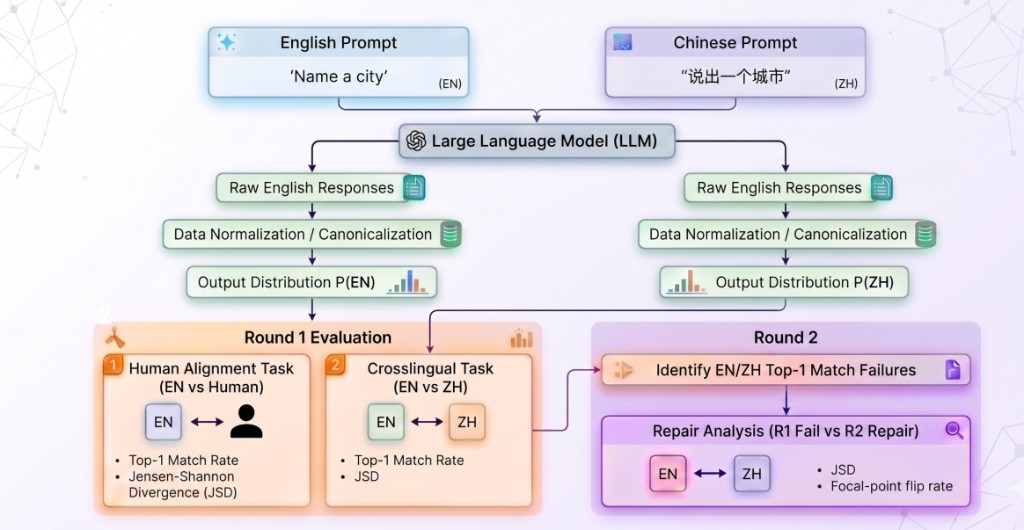
\includegraphics[width=0.88\linewidth]{evaluation_pipeline.png}
  \captionof{figure}{Overview of the human-referenced cross-lingual coordination evaluation pipeline. The protocol separates Human-vs-Model alignment from EN-vs-ZH cross-lingual stability, then runs an exploratory Round~2 retry only on first-round cross-lingual top-1 mismatch items.}
  \label{fig:pipeline}
\end{center}

For a complete Round~1 model run, we use 50 samples per item per prompt language, giving $15 \times 2 \times 50 = 1500$ raw generations. Round 2 is only run on candidate items flagged by Round 1 cross-lingual top-1 mismatch, with 10 samples per item per prompt language.

\subsection{Normalization}

The model outputs are open-ended strings, so normalization is central to the evaluation. Surface forms are mapped to canonical answers using a manually curated alias table. The alias table is not an automatic semantic clustering step: it was manually screened and verified. We only assign multiple surface forms to the same \texttt{canonical\_answer} when they are judged to be semantically equivalent for the specific item. For example, spelling variants, punctuation variants, abbreviations, or clearly identical names can be mapped together, while answers with different meanings are kept as separate canonical answers.

This manual verification matters because overly aggressive merging would artificially reduce distributional divergence. Conversely, failing to merge true variants would split probability mass across duplicate answers and inflate divergence. After normalization, invalid or unmapped responses are excluded from metric distributions. The raw data are therefore not metric values: they are model generations such as ``London'' or ``David Beckham''. Metrics such as JSD are computed only after answer normalization and distribution construction.

\subsection{Metrics}

We compute metrics at the item level and then summarize across items. Let $P$ and $Q$ be two empirical answer distributions over the same canonical answer set $\mathcal{A}$. For human alignment, $P$ is a model distribution and $Q$ is the human reference distribution. For cross-lingual stability, $P$ is the English-prompt model distribution and $Q$ is the Chinese-prompt model distribution.

\begin{itemize}[leftmargin=*]
  \item \textbf{Jensen-Shannon Divergence (JSD):}
  \[
    \operatorname{JSD}(P,Q)
    = \frac{1}{2}\operatorname{KL}(P \Vert M)
    + \frac{1}{2}\operatorname{KL}(Q \Vert M),
    \quad
    M = \frac{1}{2}(P+Q),
  \]
  where
  \[
    \operatorname{KL}(P \Vert M)
    = \sum_{a \in \mathcal{A}} P(a)\log \frac{P(a)}{M(a)}.
  \]
  JSD measures distributional divergence; lower is better.

  \item \textbf{Total Variation Distance (TVD):}
  \[
    \operatorname{TVD}(P,Q)
    = \frac{1}{2}\sum_{a \in \mathcal{A}} |P(a)-Q(a)|.
  \]
  TVD measures absolute distributional distance; lower is better.

  \item \textbf{Top-1 match:}
  \[
    \operatorname{Top1Match}(P,Q)
    =
    \mathbf{1}\left[
      \arg\max_{a \in \mathcal{A}} P(a)
      =
      \arg\max_{a \in \mathcal{A}} Q(a)
    \right].
  \]
  This is 1 if the two distributions have the same most probable canonical answer and 0 otherwise.

  \item \textbf{Flip rate:}
  \[
    \operatorname{FlipRate}(P,Q)
    = 1 - \operatorname{Top1Match}(P,Q).
  \]
  This is meaningful for cross-lingual EN/ZH comparisons, where it indicates whether the focal answer changes across instruction languages.

  \item \textbf{Spearman correlation:}
  \[
    \rho_s(P,Q)
    =
    1 - \frac{6\sum_{i=1}^{n} d_i^2}{n(n^2-1)},
  \]
  where $d_i$ is the rank difference for answer $i$ after ranking canonical answers by their probabilities in $P$ and $Q$. Higher values indicate more similar answer rankings.
\end{itemize}

For human alignment, we compare model distributions against the human reference distribution. For cross-lingual stability, we compare a model's English-prompt distribution against its Chinese-prompt distribution. The main figures and narrative emphasize JSD and top-1 match because they map directly to RQ1 and RQ2; TVD and Spearman are computed at item level for auxiliary diagnostics and exported alongside the main summaries.

\subsection{Implementation Notes}

Several design choices shaped the final protocol. We fixed the answer language to English under both English and Chinese instructions so that any shift in outputs can be attributed to instruction language rather than output language. Open-ended responses required a curated alias table and manual review; invalid and unmapped rows are excluded from all metric distributions. Human alignment (Human-vs-EN/ZH) and cross-lingual stability (EN-vs-ZH) are computed and reported separately to avoid conflating distinct evaluation targets. Reported values were traced from raw generations through normalization to aggregated metrics to confirm they are pipeline outputs rather than manual entries.

\subsection{Challenges and Solutions}
\label{sec:challenges}

\textbf{Open-ended answers and normalization.}
Models return free-text strings, but metrics require shared canonical answer keys. Early runs split probability across spelling variants and inflated JSD. We addressed this with a manually verified alias table, explicit exclusion of unmapped rows, and separation of raw generations from derived metrics so that normalization choices could be audited item by item.

\textbf{Conflating human alignment with cross-lingual stability.}
A single summary score obscured cases where a model matched humans under one prompt language but flipped focal answers across EN/ZH (or the reverse). We split the pipeline into Human-vs-model and EN-vs-ZH tracks, reported RQ1 and RQ2 on separate figures, and added item-level metric exports so that sparse flips were visible behind model-level means.

\textbf{Presentation vs.\ final figures.}
The course presentation used hand-edited slides. One slide misreported \texttt{mimo-v2-pro}'s mean \emph{cross-lingual} JSD as 0.20 (a decimal-place transcription error). This report uses only pipeline-generated tables and figures; the corrected value is 0.020 (Figure~\ref{fig:crosslingual}). For human alignment, the same model's mean top-1 match vs.\ the human reference is 0.867 in both prompt languages (Figure~\ref{fig:humanalignment}), not 0.02 or 0.20.

\section{Results and Analysis}
\label{sec:results}

We evaluate 17 Round~1 model runs on the \texttt{study2\_british\_within} panel and report exploratory Round~2 follow-up where available.

\subsection{Overview}

Figures~\ref{fig:crosslingual} and~\ref{fig:humanalignment} summarize RQ2 and RQ1, respectively (15 items, 50 samples per item per prompt language). Three patterns stand out before the detailed analyses below.

First, \textbf{cross-lingual stability is highly model-dependent} (RQ2). Mean EN-vs-ZH JSD spans roughly an order of magnitude, from 0.020 (\texttt{mimo-v2-pro}) to 0.213 (\texttt{glm-4-flashx-250414}). Second, \textbf{human alignment and cross-lingual stability decouple} (RQ1 vs.\ RQ2). The most instruction-stable models are not the closest to the human distribution; \texttt{gemini-2.5-flash} is closest to humans but still flips focal answers on 20\% of items when the prompt language changes. Third, \textbf{JSD and top-1 match tell complementary stories}: a model can preserve the same modal answer across languages while still spreading probability mass differently (nonzero JSD), or flip the focal answer on only a few items while keeping low average divergence elsewhere.

\begin{center}
  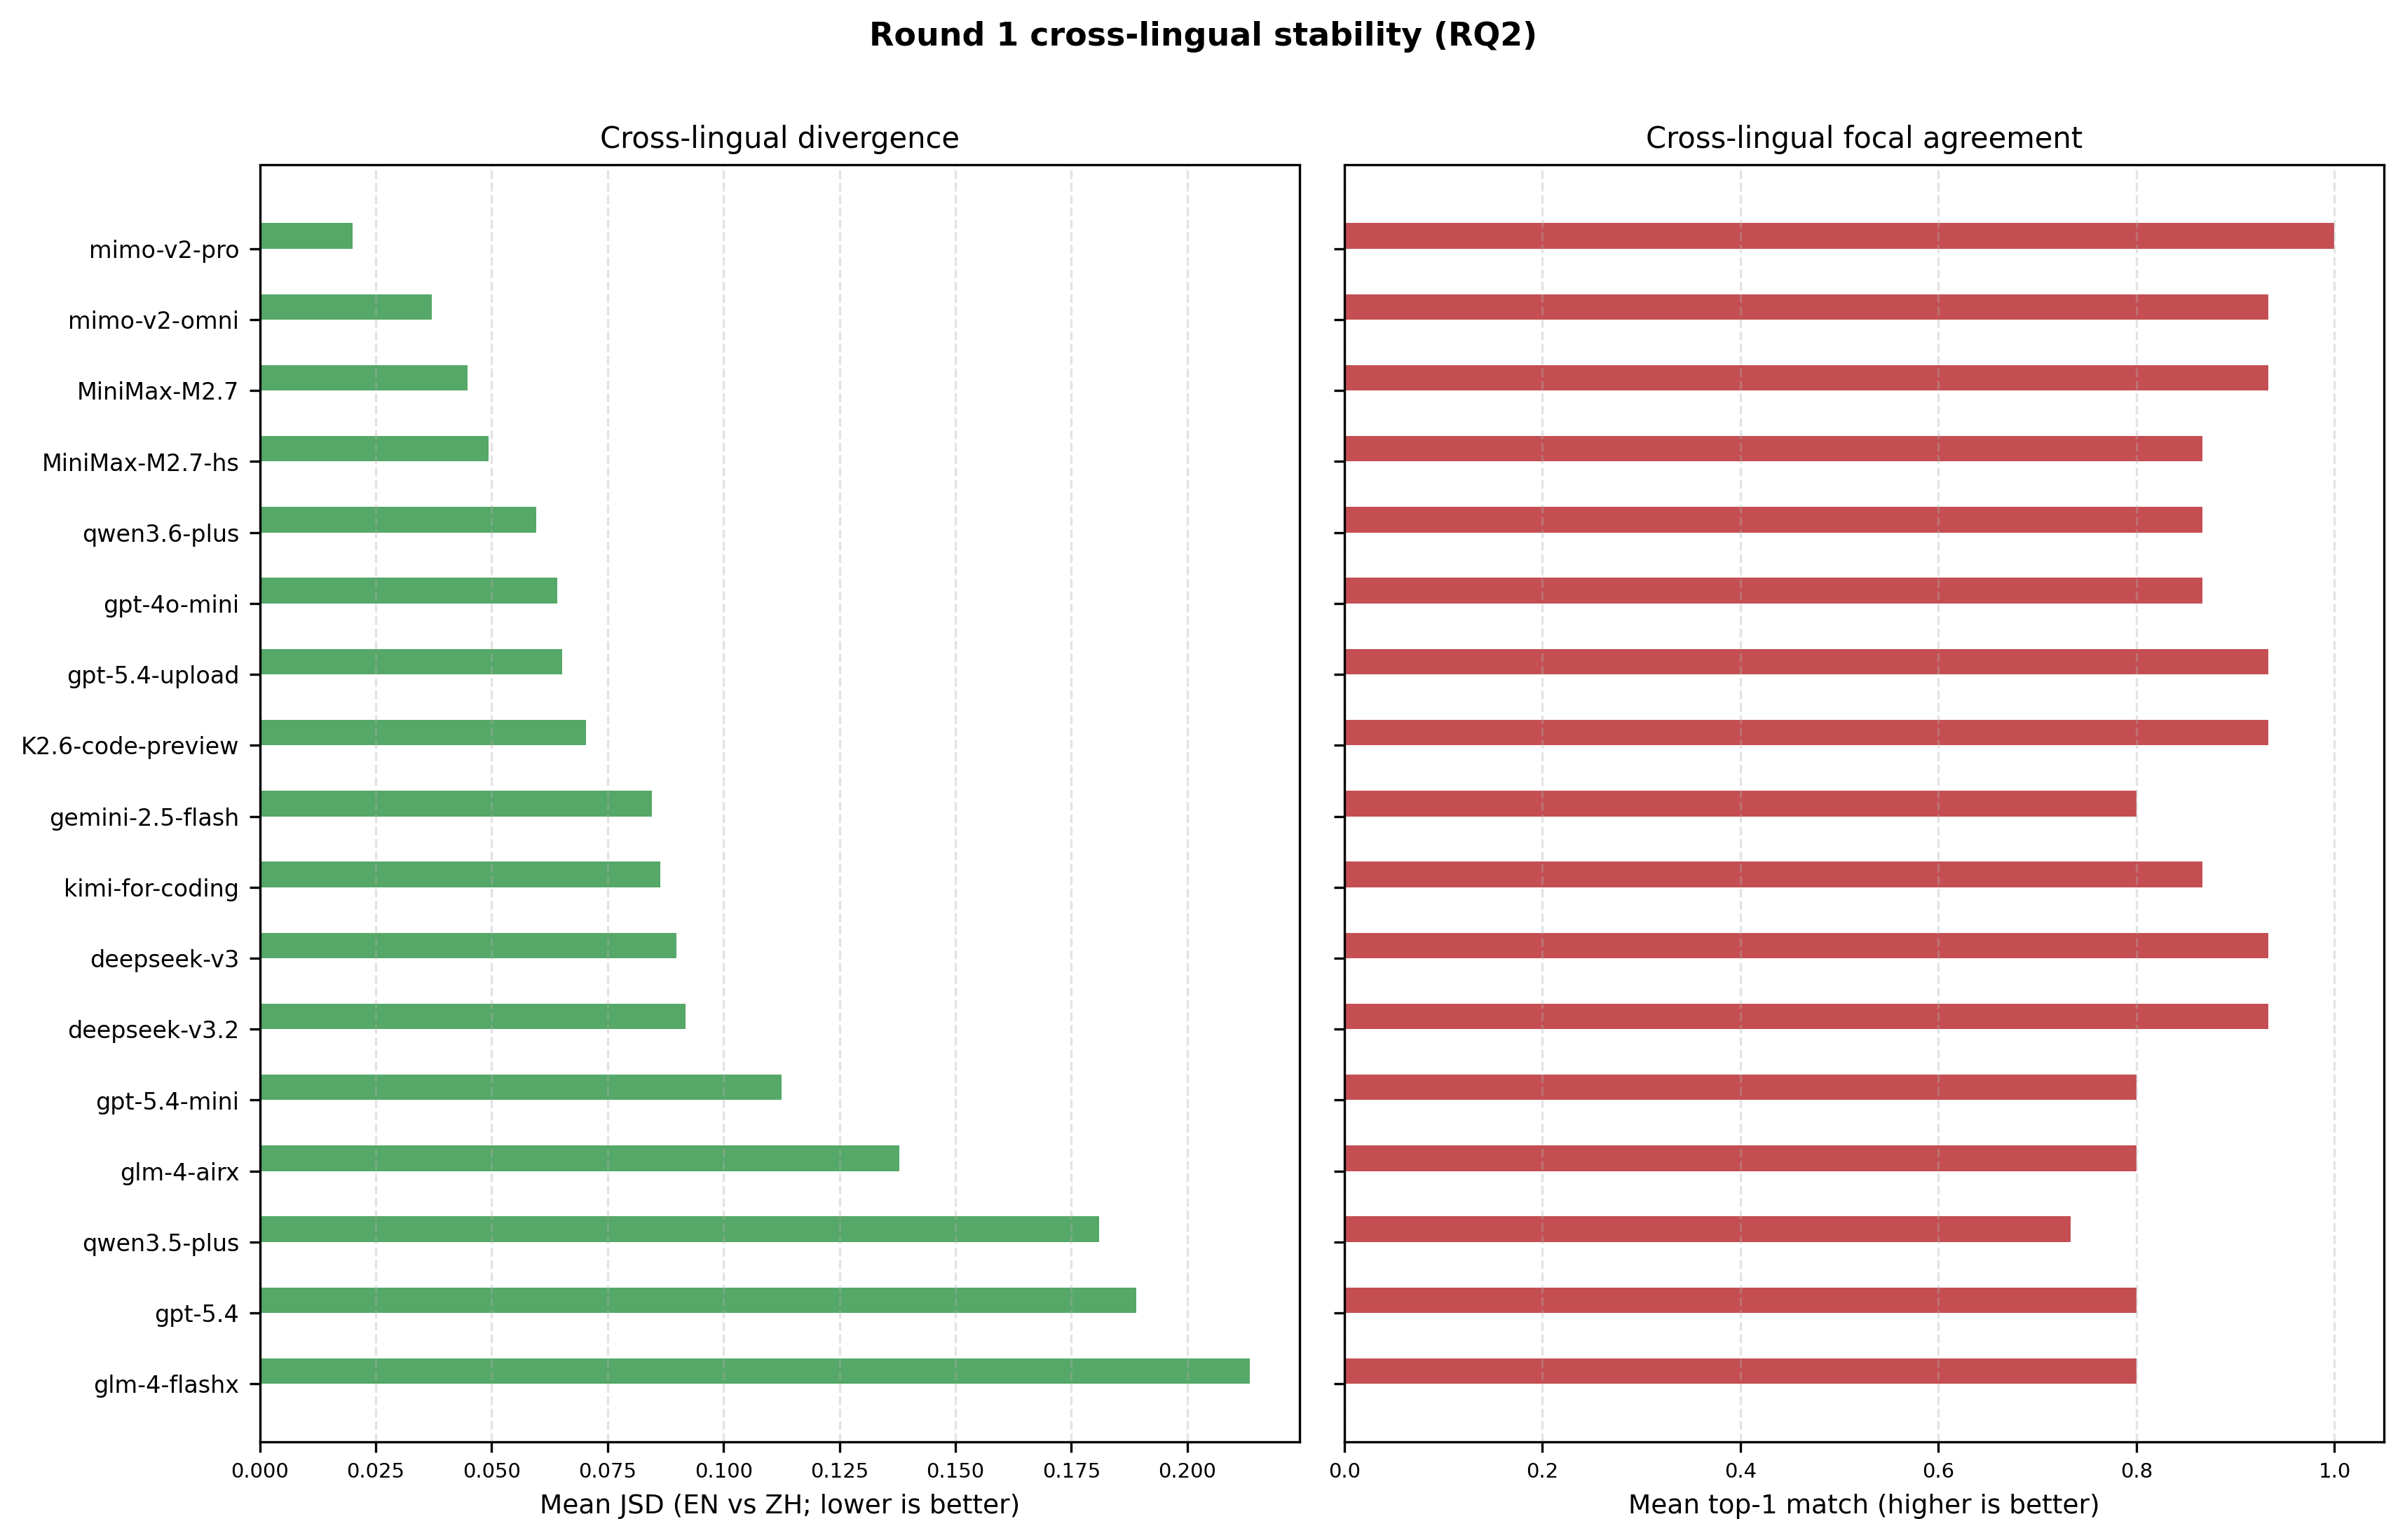
\includegraphics[width=\linewidth,height=0.26\textheight,keepaspectratio]{round1_cross_lingual_stability.png}
  \captionof{figure}{Round~1 cross-lingual stability (RQ2). Left: mean EN-vs-ZH JSD over 15 items (lower is more stable). Right: mean top-1 match between English- and Chinese-prompt distributions (higher is more stable). Models are sorted by increasing JSD.}
  \label{fig:crosslingual}
\end{center}

\subsection{Round 1 Cross-Lingual Stability (RQ2)}

Figure~\ref{fig:crosslingual} plots mean cross-lingual JSD (left) and mean top-1 match (right) for all 17 Round~1 runs. Reading the two panels together is important: JSD captures full distributional shift, whereas top-1 match only records whether the single most frequent answer is the same under English and Chinese instructions.

\paragraph{Stable tier.}
\texttt{mimo-v2-pro} is the clearest outlier on stability: mean JSD 0.020 and top-1 match 1.000, with zero flagged cross-lingual flips across all 15 items. \texttt{mimo-v2-omni} is nearly as strong (JSD 0.037, top-1 match 0.933; one mismatch item). The MiniMax M2.7 family also sits in a low-drift band (JSD 0.045--0.049, top-1 match 0.867--0.933). These models suggest that, for some LLMs, switching the instruction language while holding the answer language fixed does not materially change the emergent focal point.

\paragraph{Middle tier.}
A broad middle group---including \texttt{gpt-4o-mini}, \texttt{gpt-5.4} (round2-upload), \texttt{qwen3.6-plus}, DeepSeek v3 variants, \texttt{kimi-for-coding}, and \texttt{gemini-2.5-flash}---shows modest cross-lingual JSD (roughly 0.06--0.09) but still flips the top answer on one or two items (top-1 match 0.867--0.933). For these models, instruction language usually preserves coordination behavior, yet a minority of items drive most of the measured drift.

\paragraph{Unstable tier.}
Several models exhibit both high JSD and frequent focal flips. \texttt{qwen3.5-plus} is the weakest on top-1 agreement (0.733) with the highest flip burden (4 of 15 items) and JSD 0.181. \texttt{glm-4-flashx-250414} has the highest mean JSD (0.213) while still matching top-1 on only 80\% of items. \texttt{gpt-5.4} (main) and \texttt{glm-4-airx} show a similar pattern: JSD above 0.11--0.19 and top-1 match 0.80. Item-level diagnostics (not shown in the figure) indicate that mismatches cluster on a small set of person- and place-name items (e.g., items 3, 4, 8, and 11), where translation or cultural salience may shift which answer the model treats as the obvious focal point.

\paragraph{JSD versus top-1.}
The gap between the two panels illustrates why both metrics are needed. \texttt{gemini-2.5-flash} has moderate JSD (0.085) but top-1 match only 0.80 because three items flip; conversely, some models with top-1 match 0.93 still show nontrivial JSD when secondary answers gain or lose mass under Chinese prompts. For deployment settings where only the ``obvious'' answer matters, top-1 match is the operative criterion; for studying distributional coordination behavior, JSD is more informative.

\needspace{9\baselineskip}
\subsection{Round 1 Human Alignment (RQ1)}

\begin{center}
  \reportplot{round1_human_alignment_jsd.png}
  \captionof{figure}{Round~1 human alignment (RQ1). Grouped bars show mean Human-vs-model JSD under English prompts (blue) and Chinese prompts (orange); lower is closer to the human reference distribution.}
  \label{fig:humanalignment}
\end{center}

Figure~\ref{fig:humanalignment} compares each model's answer distribution to the human reference under English prompts (blue) and Chinese prompts (orange). Unlike Figure~\ref{fig:crosslingual}, both bars in a pair reference the \emph{same} human distribution; they differ only in which instruction language produced the model samples.

\paragraph{Closest to humans.}
\texttt{gemini-2.5-flash} achieves the lowest human-alignment JSD in both conditions (EN 0.262, ZH 0.260), indicating that its sampled distributions are the most human-like on average across the panel. \texttt{gpt-5.4-mini} (0.304 / 0.280) and the DeepSeek v3 runs (roughly 0.30--0.35 EN, lower under ZH) also sit below the bulk of the field. Notably, several models are \emph{closer} to the human distribution under Chinese instructions than under English ones (e.g., DeepSeek, \texttt{gpt-5.4-mini}, \texttt{gpt-5.4} round2-upload), even though all answers are required in English. This does not imply that Chinese prompts ``improve'' coordination in general; it shows that instruction language can shift the model toward or away from the human focal distribution depending on the model family.

\paragraph{Farthest from humans.}
\texttt{glm-4-flashx-250414} has the highest human JSD (EN 0.403, ZH 0.390), well above the cross-lingually stable \texttt{mimo-v2-pro} (0.344 / 0.316). \texttt{gpt-5.4} (main) is also human-distant under English prompts (0.386) despite improving under Chinese prompts (0.314). Thus the GLM and main GPT-5.4 runs are doubly weak on our benchmark: they drift across instruction languages \emph{and} sit far from the British-within human reference.

\paragraph{Stability $\neq$ human-likeness.}
The decoupling between RQ1 and RQ2 is the central empirical message of Figure~\ref{fig:humanalignment} when read alongside Figure~\ref{fig:crosslingual}. \texttt{mimo-v2-pro} is the most cross-lingually stable model but only mid-pack on human alignment (JSD $\approx$0.34, top-1 vs.\ human 0.867 in both languages). \texttt{qwen3.5-plus} has relatively strong human top-1 match under English prompts (0.867) yet the worst cross-lingual top-1 match (0.733) because Chinese prompts shift its focal answers on four items. \texttt{gpt-5.4} (main) shows the reverse asymmetry: poor cross-lingual stability but the highest human top-1 match under Chinese prompts (0.933). A single leaderboard score cannot summarize tacit coordination behavior; practitioners need both human-referenced and cross-lingual diagnostics.

\paragraph{Instruction-language effects on human match.}
For most models, EN and ZH human-alignment JSD differ by only 0.01--0.04, suggesting that the dominant factor is model identity rather than prompt language. Exceptions matter: \texttt{MiniMax-M2.7-highspeed} and \texttt{kimi-for-coding} show larger EN--ZH gaps in human JSD, and \texttt{gpt-5.4} (main) improves markedly under Chinese instructions. These cases reinforce that translation of the task stem is not a neutral re-labeling: it can change which human-like focal point the model approximates, independent of whether EN and ZH prompts agree with each other. On the human axis, modal agreement (top-1 vs.\ human) and full distributional closeness (JSD) can also diverge, as with \texttt{gpt-5.4} (main) under Chinese prompts.

\subsection{Round 2 Candidate Items (Exploratory, RQ3)}

Round~2 is triggered only when Round~1 shows a cross-lingual top-1 mismatch on an item. Each baseline model then receives the lightweight second-round retry prompt on \emph{its own} flagged items (10 samples per language), which tests RQ3---whether the original model can recover focal agreement---without rerunning the full 15-item panel.

All Round~2 summaries are \textbf{paired on the same candidate items}: for each model, we compare Round~1 and Round~2 cross-lingual metrics only over items that already mismatched in Round~1 (typically $n=1$--$4$, annotated in the figures).

\needspace{8\baselineskip}
\begin{center}
  \reportplot{strict_permodel_same_item_improvement_pct.png}
  \captionof{figure}{Round~2 vs.\ Round~1 on the same candidate items (RQ3). Green: share of flagged items with lower cross-lingual JSD; red: share with restored top-1 agreement (Round~1 top-1 was 0 on these items). The dashed line marks 50\%.}
  \label{fig:r2-improve}
\end{center}

Figure~\ref{fig:r2-improve} reports, for each model, the percentage of its flagged items with lower cross-lingual JSD (green) and with restored top-1 agreement (red). \texttt{qwen3.5-plus} improves on all four candidates for JSD (100\% green) and on three of four for top-1 (75\% red). \texttt{qwen3.6-plus}, \texttt{gpt-5.4-mini}, \texttt{gemini-2.5-flash}, \texttt{mimo-v2-omni}, \texttt{MiniMax-M2.7}, and \texttt{K2.6-code-preview} show majority improvement on at least one metric. At the other extreme, \texttt{deepseek-chat} (both runs), \texttt{glm-4-flashx-250414}, and \texttt{glm-4-airx} show \textbf{0\%} top-1 recovery; GLM lines still show partial JSD reduction (green) without modal realignment. \texttt{gpt-5.4} (main runs) lowers JSD on about half of flagged items but does not restore top-1 on any.

\needspace{8\baselineskip}
\begin{center}
  \reportplot{strict_permodel_same_items_r1_r2_jsd.png}
  \captionof{figure}{Round~2 (RQ3): mean cross-lingual JSD on the same candidate items as Round~1 (lower is better). Round~1 values are high because these items were selected for mismatch; the drop in orange bars quantifies distributional recovery.}
  \label{fig:r2same-jsd}
\end{center}

Figure~\ref{fig:r2same-jsd} adds distributional detail. \texttt{qwen3.5-plus} drops from mean JSD 0.59 to 0.07 on its four candidates, including item~4 where Round~1 exhibited a complete focal flip (JSD up to 1.0). \texttt{gpt-5.4-mini} and \texttt{qwen3.6-plus} show similar JSD reductions. Several models lower JSD without gaining top-1 (e.g., \texttt{gpt-5.4} on three items), meaning drift shrinks but the EN/ZH modal answers can remain different.

Across 31 item-level pairs, Round~2 restores top-1 on \textbf{14} (45\%), lowers JSD on \textbf{21} (68\%), and achieves both on \textbf{14}. Eight of fifteen models improve \emph{both} mean top-1 and mean JSD on their candidate sets.

\paragraph{RQ3 assessment.}
These results are \textbf{partially positive} for RQ3: a lightweight retry can fix many, but not all, cross-lingual mismatches. Recovery is strongly model-dependent (helpful for Qwen and some GPT/Gemini runs; largely ineffective for GLM, DeepSeek, and main \texttt{gpt-5.4}). Round~2 remains exploratory because candidate counts are small and sampling uses 10 draws per language.

\subsection{Discussion}
\label{sec:discussion}

\paragraph{Interpretation.}
Our results support a diagnostic rather than monolithic view of LLM coordination. Tacit coordination in LLMs is not one capability but (at least) two: matching a human reference distribution, and remaining consistent when the instruction language changes while the answer language is fixed. The benchmark makes these axes measurable on the same items and sampling budget.

\paragraph{Why some models flip on specific items.}
Cross-lingual mismatches are sparse but structured. Flagged items often involve entities where British and translated prompts may prime different salient answers (people, places, brands). On item~4, for example, \texttt{qwen3.5-plus} can assign essentially all English-prompt mass to one focal answer and essentially all Chinese-prompt mass to another (item-level JSD up to 1.0), even when the other 14 items are stable. A single such flip is enough to pull down mean top-1 match; this argues for reporting both item-level and model-level views, not only means over 15 items.

\paragraph{Mechanistic hypotheses (speculative).}
We do not identify causal mechanisms, but several patterns are plausible. Cross-lingually stable yet human-distant models (e.g., \texttt{mimo-v2-pro}) may rely on strong internal defaults that are insensitive to instruction translation but misaligned with a British-within human panel. Human-aligned yet instruction-sensitive models (e.g., \texttt{gemini-2.5-flash}) may track human salience under English prompts while Chinese stems re-weight entity names or categories in the translated item text. Models with high human top-1 under one language only (e.g., \texttt{gpt-5.4} main) may be optimizing a different apparent focal point when the stem language changes, even while answers remain in English. These hypotheses could be tested with ablations on translation quality, panel country, answer-language variation, and language-confusion controls \cite{marchisio2024language}.

\paragraph{Implications for deployment.}
For applications that require consistent behavior under multilingual UI or prompts, the stable tier (\texttt{mimo-v2-pro}, \texttt{mimo-v2-omni}, parts of the MiniMax line) is preferable. For applications that require human-like focal points on this British panel, \texttt{gemini-2.5-flash} and some GPT/DeepSeek variants are stronger choices despite weaker cross-lingual robustness. No evaluated model dominates both criteria.

\paragraph{Multi-agent routing.}
Round~1 does not measure coordination \emph{between} models, but the decoupling of RQ1 and RQ2 already constrains how one might compose teams. A pipeline that mixes a human-aligned planner with a cross-lingually stable executor, or that routes multilingual UI traffic only through stable models, is more consistent with the data than assuming one ``best'' model for every agent role. Future inter-model batteries (Section~\ref{sec:futurework}) are needed before claiming efficiency gains in real multi-agent systems.

\paragraph{Relation to prior work.}
Classical focal-point theory and experiments \cite{schelling1960,mehta1994,sugden1995} justify distributional comparison on canonical answers. Perez-Zapata et al.\ establish cross-cultural variation in \emph{human} focal points across panels \cite{perez2026}; we hold the human reference fixed and stress-test \emph{LLM} instruction-language sensitivity on the same items. Aharon et al.\ and Agashe et al.\ establish that LLMs can coordinate in game-like settings \cite{aharon2026,agashe2025coord}; we ask whether single-model focal points are \emph{stable} when only the instruction language changes. Marchisio et al.\ warn that multilingual prompts can shift model behavior in hard-to-predict ways \cite{marchisio2024language}, consistent with the item-level flips we observe. The contribution is diagnostic: human-comparison metrics also separate cross-lingual stability, and those axes need not move together.

\paragraph{Caveats.}
All Round~1 findings are tied to one panel, English answer language, 50 samples per item per language, and a curated alias table; model rankings could shift with more samples or bootstrap intervals. JSD values in the 0.25--0.40 range for human alignment indicate substantial remaining divergence from humans even for the best models. We do not interpret Chinese prompts as a proxy for Chinese culture, and we do not treat cross-lingual stability as evidence about reasoning depth or theory of mind. Round~2 is paired on candidate items only, uses fewer samples than Round~1, and does not repair all flagged flips; it should not be pooled with Round~1 as a universal intervention.

\section{Conclusion}
\label{sec:conclusion}

This project delivers a reproducible diagnostic pipeline for cross-lingual tacit coordination in LLMs. Round~1 results (Figures~\ref{fig:crosslingual} and~\ref{fig:humanalignment}) show substantial heterogeneity: \texttt{mimo-v2-pro} is the most instruction-stable model, \texttt{gemini-2.5-flash} is closest to the human reference on this panel, and no model leads on both axes. Section~\ref{sec:discussion} argues that these are separable capabilities with distinct deployment implications, including cautious multi-agent routing based on role rather than a single leaderboard. Round~2 (Figures~\ref{fig:r2-improve} and~\ref{fig:r2same-jsd}) partially supports RQ3: many mismatches are prompt-sensitive for some model families, but not for others.

\subsection{Reflection and Learning}
\label{sec:reflection}

Evaluating tacit coordination in LLMs is as much a data-engineering problem as a modeling problem. The most important lesson was to keep raw generations, normalized answers, and summary metrics in separate artifacts so that each stage could be checked independently. Normalization and alias coverage were not cosmetic preprocessing; they changed which models looked stable or human-like.

Separating human alignment from cross-lingual stability was the second lesson. Collapsing RQ1 and RQ2 into one score would have hidden the central empirical finding---that no evaluated model leads on both axes---and would have misled deployment recommendations for multilingual or multi-agent settings.

Packaging the workflow as \texttt{coordbench} with YAML configs and provider adapters made it practical to rerun panels and add Round~2 follow-up without one-off scripts.

\subsection{Limitations}
\label{sec:limitations}

The current finalized analysis uses one human panel, \texttt{study2\_british\_within}, so the results should not be framed as a broad cross-cultural conclusion. The Chinese condition changes the instruction language, but the answer language remains English; this isolates one design factor but does not causally separate language, culture, and translation effects.

Normalization is another limitation. Alias rules make the benchmark possible, but they also introduce measurement choices. We reduced this risk through manual alias cleanup and by excluding invalid or unmapped outputs, but normalization remains a source of uncertainty.

Round~2 is candidate-only and uses 10 samples per language (versus 50 in Round~1). Each model is rerun on only its own 1--4 flagged items, so item-level improvement rates are noisy.

\subsection{Future Work}
\label{sec:futurework}

\paragraph{Benchmark extensions.}
Future work could extend the panel to more countries, instruction languages, and human reference distributions \cite{perez2026}. A stronger design would also vary answer language directly, separating instruction-language effects from output-language effects. Round~2 should be extended with larger per-item sample sizes and bootstrap intervals on candidate subsets.

\paragraph{Inter-model and within-family coordination.}
The current study evaluates each model in isolation. A natural next step is to measure \emph{coordination between} models: for the same item, compare the answer distributions of model~A and model~B (JSD, top-1 match) and ask whether models from the same family, vendor, or parameter scale cluster together. Systematic comparisons across model series (e.g., \texttt{mimo-v2-pro} vs.\ \texttt{mimo-v2-omni}), sizes, and training regimes would test whether ``more coordinate'' pairings exist---a question we do not answer in Round~1.

\paragraph{Multi-agent deployment efficiency.}
An applied follow-up could pair high- and low-agreement model teams on a shared coordination-item battery, then embed those teams in realistic multi-agent pipelines (planning, code generation, or tool use). Outcomes might include conflict rate, number of repair rounds, and human edit distance. Such experiments could test whether composing models with high mutual focal-point agreement---and separately considering human alignment vs.\ cross-lingual stability when choosing roles---reduces coordination overhead relative to heterogeneous low-agreement teams. This remains a hypothesis: we do not claim that high-agreement combinations are already more efficient.

\paragraph{Heterogeneous team design.}
Because no evaluated model dominates both human alignment and cross-lingual stability, future work could explore deliberate role splits (e.g., a human-aligned model for user-facing suggestions and a cross-lingually stable model for multilingual interfaces) rather than assuming one model fits all agents in a pipeline.

\paragraph{Engineering.}
Plotting, normalization, and metric scripts should receive stronger regression tests so that column-mapping and alias-coverage mistakes are caught automatically before they affect reported figures.

\section{References}

\begin{thebibliography}{99}

\bibitem{aharon2026}
Aharon, I., La Malfa, E., Wooldridge, M., and Kraus, S. (2026).
\newblock Tacit Coordination of Large Language Models.
\newblock \textit{arXiv:2601.22184}.
\newblock \url{https://arxiv.org/abs/2601.22184}.

\bibitem{agashe2025coord}
Agashe, S., Fan, Y., Reyna, A., and Wang, X. E. (2025).
\newblock LLM-Coordination: Evaluating and Analyzing Multi-agent Coordination Abilities in Large Language Models.
\newblock In \textit{Findings of the Association for Computational Linguistics: NAACL 2025}, pages 8053--8072.
\newblock \url{https://aclanthology.org/2025.findings-naacl.448/}.

\bibitem{marchisio2024language}
Marchisio, K., Ko, W.-Y., Berard, A., Dehaze, T., and Ruder, S. (2024).
\newblock Understanding and Mitigating Language Confusion in LLMs.
\newblock In \textit{Proceedings of the 2024 Conference on Empirical Methods in Natural Language Processing}, pages 6653--6677.
\newblock \url{https://aclanthology.org/2024.emnlp-main.380/}.

\bibitem{mehta1994}
Mehta, J., Starmer, C., and Sugden, R. (1994).
\newblock The Nature of Salience: An Experimental Investigation of Pure Coordination Games.
\newblock \textit{American Economic Review}, 84(3), 658--673.

\bibitem{perez2026}
Perez-Zapata, D., Isoni, A., Zawidzki, T., and Apperly, I. (2026).
\newblock Three International Studies on Pure Coordination Games: Adaptable Solutions When Intuitions are Presumed to Vary.
\newblock \textit{Journal of Experimental Psychology: General}, 155(3), 760--775.
\newblock \url{https://doi.org/10.1037/xge0001876}.

\bibitem{schelling1960}
Schelling, T. C. (1960).
\newblock \textit{The Strategy of Conflict}.
\newblock Harvard University Press.

\bibitem{sugden1995}
Sugden, R. (1995).
\newblock A Theory of Focal Points.
\newblock \textit{The Economic Journal}, 105(430), 533--550.
\newblock \url{https://doi.org/10.2307/2235016}.

\end{thebibliography}

\appendix
\renewcommand{\thesection}{Appendix:}
\setcounter{section}{0}
\section{Reproducibility Pointers}

The main report figures were generated from the CSV files in \texttt{results/final\_project\_tables/} using \texttt{tools/plot\_final\_report\_round1.py}. Full numeric exports and item-level breakdowns are in \texttt{docs/final\_project\_model\_results\_tables.md} and the same CSV directory. The key raw and intermediate run artifacts are:

\begin{itemize}[leftmargin=*]
  \item \texttt{raw\_generations.jsonl}: raw model responses;
  \item \texttt{normalized\_outputs.csv}: normalized canonical answers;
  \item \texttt{item\_metrics.csv}: item-level JSD, TVD, top-1 match, flip rate, and Spearman;
  \item \texttt{summary\_metrics.json}: model-level summaries;
  \item \texttt{round2\_candidates.csv}: Round 1 cross-lingual mismatch candidates;
  \item \texttt{results/final\_project\_tables/}: Round~1 tables plus paired Round~1/2 item metrics for Round~2 reruns;
  \item \texttt{tools/plot\_strict\_permodel\_r1\_r2.py}: generates Round~2 summary figures used in the report.
\end{itemize}

\end{document}
